\title{Combinational Circuits}
\begin{document}
\section{Switching (Boolean) Algebra}
\subsection{Axioms}

\begin{frame}{The uncaused Cause}
  \begin{definition}
    An \alert{axiom} is a statement that is assumed to be true.
  \end{definition}
  \begin{block}{Axioms of Switching Algebra (George Boole's Top Ten List)}
    \begin{center}
      \begin{tabular}{llll}
        (A1) & $X=0$ if $X \neq 1$ & (A1$'$) & $X=1$ if $X \neq 0$ \\
        (A2) & If $X=0$, then $X'=1$ & (A2$'$) & If $X=1$, then $X'=0$ \\
        (A3) & $0 \cdot 0 = 0$ & (A3$'$) & $1 + 1 = 1$ \\
        (A4) & $1 \cdot 1 = 1$ & (A4$'$) & $0 + 0 = 0$ \\
        (A5) & $0 \cdot 1 = 1 \cdot 0 = 0$ & (A5$'$) & $1 + 0 = 0 + 1 = 1$ \\
      \end{tabular}
    \end{center}
  \end{block}
  \begin{itemize}
    \item The unary \alert{complement} operator $'$ is spelled ``prime'' or ``not''.
    \item The binary \alert{logical multiplication} operator $\cdot$ is spelled ``and''.
    \item The binary \alert{logical addition} operator $+$ is spelled ``or''.
    \item Precedence is$'$,$\cdot$,$+$: $X \cdot Y + Z = (X \cdot Y) + Z$.
  \end{itemize}
\end{frame}

\begin{itemize}
  \item All mathematical systems have axioms - take Euclidean geometry - parallel lines never intersect.  This is not true in other geometries.
\end{itemize}

\subsection{Duality}

\begin{frame}{Duality}
  \begin{block}{Principle of Duality (pg 193 of Wakerly)}
    Any theorem or identity in switching algebra remains true if 0 and 1 are swapped and $\cdot$ and $+$ are swapped throughout.
  \end{block}
  \begin{definition}
    The \alert{dual of a logic expression} $F(X_1, X_2, \ldots, X_n, +, \cdot, ')$ where $X_1, X_2, \ldots, X_n$ are variables and $+,\cdot,'$ are operators is $F^D(X_1, X_2, \ldots, X_n, \cdot, +, ')$.
  \end{definition}
  The principle of duality follows from the ten axioms, which are really a set of five duals.
\end{frame}

\subsection{Useful Theorems}

\begin{frame}{Single-variable theorems}
  \begin{block}{Single-Variable Theorems (Table 4-1 pg 188 of Wakerly)}
    \begin{center}
      \begin{tabular}{lllll}
        (T1) & $X + 0 = X$ & (T1$'$) & $X \cdot 1 = X$ & Identities \\
        (T2) & $X + 1 = 1$ & (T2$'$) & $X \cdot 0 = 0$ & Null elements \\
        (T3) & $X + X = X$ & (T3$'$) & $X \cdot X = X$ & Idempotency \\
        (T4) & $(X')' = X$ & & & Involution \\
        (T5) & $X + X' = 1$ & (T5$'$) & $X \cdot X' = 0$ & Complements\\
      \end{tabular}
    \end{center}
  \end{block}
  \begin{itemize}
    \item Unlike those messy infinite systems like integers or real numbers, we only have two possible values for $X$, 0 and 1.
    \item These theorems can all be proven by \alert{perfect induction} - simply test them for all possible values of $X$.
    \item Notice the duality.
  \end{itemize}
\end{frame}

\begin{frame}{Two- and three-variable theorems}
  \begin{block}{Two- and Three-Variable Theorems (Table 4-2 pg 189 of Wakerly)}
    \begin{center}
      \begin{tabular}{ll}
        (T6) Commutativity & $X + Y = Y + X$ \\
        (T6$'$) & $X \cdot Y = Y \cdot X$ \\
        (T7) Associativity & $(X + Y) + Z = X + (Y + Z)$ \\
        (T7$'$) & $(X \cdot Y) \cdot Z = X \cdot (Y \cdot Z)$ \\
        (T8) Distributivity& $X \cdot Y + X \cdot Z = X \cdot (Y + Z)$ \\
        (T8$'$) & $(X + Y) \cdot (X + Z) = X + Y \cdot Z$ \\
        (T9) Covering & $X + X \cdot Y = X$ \\
        (T9$'$) & $X \cdot (X + Y) = X$ \\
        (T10) Combining & $X \cdot Y + X \cdot Y' = X$ \\
        (T10$'$) & $(X + Y) \cdot (X + Y')=X$ \\
        (T11) Consensus & $X \cdot Y + X' \cdot Z = Y \cdot Z = X \cdot Y + X' \cdot Z$ \\
        (T11$'$) & $(X + Y) \cdot (X' + Z) \cdot (Y+Z)$ \\
                 & $ = (X + Y) \cdot (X' + Z)$ \\
      \end{tabular}
    \end{center}
  \end{block}
\end{frame}

\begin{itemize}
  \item Theorems (T6) and (T7) (and their duals) are very important, because they allow us to rearrange inputs to gates and use gates with more than two inputs.
  \item Notice (T8$'$) - we can distribute logical addition over logical multiplication.
  \item These theorems can also be proven by perfect induction.
\end{itemize}

\begin{frame}{$n$-Variable theorems}
  \begin{block}{$n$-Variable Theorems (Table 4-3 pg 191 of Wakerly)}
    Generalized idempontency \\
    \begin{tabular}{ll}
      (T12) & $X + X + \cdots + X = X$ \\
      (T12$'$) & $X \cdot X \cdot \cdots \cdot X = X$ \\
    \end{tabular} \\
    DeMorgan's theorems \\
    \begin{tabular}{ll}
      (T13) & $(X_1 \cdot X_2 \cdot \cdots \cdot X_n)' = X_1' + X_2' + \cdots + X_n'$ \\
      (T13$'$) & $(X_1 + X_2 + \cdots + X_n)' = X_1' \cdot X_2' \cdot \cdots \cdot X_n'$ \\
    \end{tabular} \\
    Generalized DeMorgan's theorem \\
    \begin{tabular}{ll}
      (T14) & $[F(X_1, X_2, \ldots, X_n, +, \cdot)]' = F(X_1', X_2', \ldots, X_n', \cdot, +)$ \\
    \end{tabular} \\
    Shannon's expansion theorems \\
    \begin{tabular}{ll}
      (T15) & $F(X_1, X_2, \ldots, X_n)$ \\ 
            & $= X_1 \cdot F(1, X_2, \ldots, X_n) + X_1' \cdot F(0, X_2, \ldots, X_n)$ \\
      (T15$'$) & $F(X_1, X_2, \ldots, X_n)$ \\ 
               & $= [X_1 + F(0, X_2, \ldots, X_n)] \cdot [X_1' + F(1, X_2, \ldots, X_n)]$ \\
    \end{tabular}
  \end{block}
\end{frame}

\subsection{Representation of Logic Functions}

\begin{frame}{Switching algebra lingo}
  \begin{block}{Sum-of-products Expression}
    $X \cdot Y + Z \cdot X' + Y \cdot Z$
  \end{block}
  \begin{block}{Product-of-sums Expression}
    $(X + Y) \cdot (Z + X') \cdot (Y + Z)$
  \end{block}
  \begin{block}{Minterm}
    A minterm is a product term that is 1 in exactly one row of a given truth table.
  \end{block}
  \begin{block}{Maxterm}
    A minterm is a sum term that is 0 in exactly one row of a given truth table.
  \end{block}
\end{frame}

\begin{frame}{The truth table revisited}
  \begin{tabular}{c|ccc|c|cc}
    \textbf{Row} & \textbf{$X$} & \textbf{$Y$} & \textbf{$Z$} & \textbf{F} & \textbf{Minterm} & \textbf{Maxterm} \\
    \hline
     0 & 0 & 0 & 0 & F(0,0,0) & $X' \cdot Y' \cdot Z'$ & $X + Y + Z$ \\
     1 & 0 & 0 & 1 & F(0,0,1) & $X' \cdot Y' \cdot Z$ & $X + Y + Z'$ \\
     2 & 0 & 1 & 0 & F(0,1,0) & $X' \cdot Y \cdot Z'$ & $X + Y' + Z$ \\
     3 & 0 & 1 & 1 & F(0,1,1) & $X' \cdot Y \cdot Z$ & $X + Y' + Z'$ \\
     4 & 1 & 0 & 0 & F(1,0,0) & $X \cdot Y' \cdot Z'$ & $X' + Y + Z$ \\
     5 & 1 & 0 & 1 & F(1,0,1) & $X \cdot Y' \cdot Z$ & $X' + Y + Z'$ \\
     6 & 1 & 1 & 0 & F(1,1,0) & $X \cdot Y \cdot Z'$ & $X' + Y' + Z$ \\
     7 & 1 & 1 & 1 & F(1,1,1) & $X \cdot Y \cdot Z$ & $X' + Y' + Z'$ \\
  \end{tabular}
\end{frame}

\begin{frame}{Converting a truth table into a logic function}
  \begin{columns}
    \begin{column}{3cm}
      Determine F: \\
      \medskip
      \begin{tabular}{c|ccc|c}
        \textbf{Row} & \textbf{$X$} & \textbf{$Y$} & \textbf{$Z$} & \textbf{F} \\
        \hline
         0 & 0 & 0 & 0 & 0 \\
         1 & 0 & 0 & 1 & 0 \\
         2 & 0 & 1 & 0 & 1 \\
         3 & 0 & 1 & 1 & 0 \\
         4 & 1 & 0 & 0 & 1 \\
         5 & 1 & 0 & 1 & 1 \\
         6 & 1 & 1 & 0 & 1 \\
         7 & 1 & 1 & 1 & 1 \\
      \end{tabular}
    \end{column}
    \begin{column}{7cm}
      \begin{itemize}
        \item The \alert{canonical sum} is the sum of minterms which produce a 1: $F = \sum_{X,Y,X}(2,4,5,6,7) = X' \cdot Y \cdot Z' + X \cdot Y' \cdot Z' + X \cdot Y' \cdot Z + X \cdot Y \cdot Z' + X \cdot Y \cdot Z$
        \item The \alert{canonical product} is the product of the maxterms which produce a 0: $F=\prod_{X,Y,Z}(0,1,3) = (X + Y + Z) \cdot (X + Y + Z') \cdot (X + Y' + Z')$
      \end{itemize}
    \end{column}
  \end{columns}
\end{frame}

\section{Combinational Circuit Analysis}

\begin{frame}{Analyze This (The Billy Crystal section)}
  \begin{block}{Why do we perform combinational circuit analysis?}
    Given a logic circuit, we analyze it by determining its logic function.
    \begin{itemize}
      \item This will allow us to determine the behavior of the circuit for any input combination.
      \item We may be able to simplify the circuit to more efficiently perform the same logic function.
      \item We can transform the logic function into a standard form (sum-of-products or product-of-sums)
      \item We can use the logic function to determine the behavior of the circuit in a larger circuit.
    \end{itemize}
  \end{block}
\end{frame}

\begin{frame}{This isn't the stand up comedy circuit}
  Determine the logic function for this logic circuit:\\
  \begin{center}
    \includegraphics{AnalysisLogicDiagram}
  \end{center}
\end{frame}

\subsection{Brute Force Analysis}

\begin{frame}{You are the brute squad.}
  We can write every input combination for each gate, then create a truth table and use the canonical approaches to determine the logic function.\\
  \begin{center}
    \includegraphics{AnalysisLogicDiagramAllInputs}
  \end{center}
\end{frame}

\subsection{The Algebraic Technique}

\begin{frame}{Whose idea was this anyway?}
  Instead, we can use the algebraic technique to write the value of each signal in switching algebra notation.\\
  \begin{center}
    \includegraphics{AnalysisLogicDiagramBooleanAlgebra}
  \end{center}
\end{frame}

\subsection{Circuit Simplification}

\begin{frame}{Very strangely they say.}
  So we have the following logic function for this circuit:\\
  \begin{tabular}{rl}
    $F$ & $= X' \cdot Y' + (X' + Z')'$ \\
        & $=X' \cdot Y' + (X \cdot Z)$ \\
  \end{tabular}\\
  Which can be written using only five gates:\\
  \begin{center}
    \includegraphics{AnalysisLogicDiagramSimplified}
  \end{center}
\end{frame}

\begin{itemize}
  \item Note that this is the sum of products representation of the logic function.
  \item The product of sums form is $F = (X' + Z) \cdot (Y' + X) \cdot (Y' + Z)$.
\end{itemize}

\section{Combinational Circuit Synthesis}

\subsection{Circuit Descriptions}

\begin{frame}{English - the language of circuit design}
  Since we want a circuit that does something useful, it usually easiest to describe that circuits behavior in English.
  \begin{block}{The Roommate Control Circuit}
    Suppose your roommate snores.  Let's design a circuit to deal with that.\\
    ``If my roommate is snoring and I need quiet, throw a shoe at him, unless he has a test tomorrow.''\\
    ``I need quiet when I'm studying or watching Top Gun.''
  \end{block}
  SHOE = SNORING $\cdot$ QUIET $\cdot$ TEST$'$ \\
  QUIET = STUDYING + MAVERICK \\
  SHOE = SNORING $\cdot$ (STUDYING + MAVERICK) $\cdot$ TEST$'$ 
\end{frame}

\begin{frame}{The roommate control circuit}
  \begin{center}
    \includegraphics[scale=1.5]{RoommateControlCircuit}
  \end{center}
\end{frame}

\subsection{Conversion to NAND and NOR Gates}

\begin{frame}{Design trade-offs}
  \begin{itemize}
    \item Recall that the CMOS implementation of the logic gates NAND and NOR was much simpler and faster than the AND or OR implementation.
    \item However, we don't usually think in terms of NAND and NOR, we think in terms of AND and OR.
    \item Wouldn't it be nice if we could map AND and OR gates to NAND and NOR gates?
  \end{itemize}
\end{frame}

\begin{frame}{Another look at sum-of-products}
  \begin{columns}
    \begin{column}[t]{5cm}
      Sum-of-products logic gates: \\
      \begin{center}
        \includegraphics{ANDOR}
      \end{center}
      Simplifies to: \\
      \begin{center}
        \includegraphics{NANDNAND}
      \end{center}
    \end{column}
    \begin{column}[t]{5cm}
      Add extra inverters: \\
      \begin{center}
        \includegraphics{ANDNOTNOTOR}
      \end{center}
      NOT-OR = NAND: \\
      \begin{center}
        \begin{tabular}{ccc}
          \textbf{X} & \textbf{Y} & \textbf{F} \\
          \hline
          0 & 0 & 1 \\
          0 & 1 & 1 \\
          1 & 0 & 1 \\
          1 & 1 & 0 \\
        \end{tabular}
      \end{center}
    \end{column}
  \end{columns}
\end{frame}

\begin{frame}{The same is true for product-of-sums}
  \begin{columns}
    \begin{column}[t]{5cm}
      Product-of-sums logic gates: \\
      \begin{center} 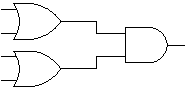
\includegraphics{ORAND}
      \end{center}
      Simplifies to: \\
      \begin{center}
        \includegraphics{NORNOR}
      \end{center}
    \end{column}
    \begin{column}[t]{5cm}
      Add extra inverters: \\
      \begin{center}
        \includegraphics{ORNOTNOTAND}
      \end{center}
      NOT-AND = NOR: \\
      \begin{center}
        \begin{tabular}{ccc}
          \textbf{X} & \textbf{Y} & \textbf{F} \\
          \hline
          0 & 0 & 1 \\
          0 & 1 & 0 \\
          1 & 0 & 0 \\
          1 & 1 & 0 \\
        \end{tabular}
      \end{center}
    \end{column}
  \end{columns}
\end{frame}

\subsection{Minimization with Karnaugh Maps}

\begin{frame}{Karnaugh maps (K maps)}
  Karnaugh maps provide a graphical way to visualize a truth table using minterms (sum-of-products).\\
  \begin{center}
    \begin{tabular}{ccc}
      \includegraphics[scale=0.5]{2VariableKMap} & \includegraphics[scale=0.5]{3VariableKMap} & \includegraphics[scale=0.5]{4VariableKMap} \\
    \end{tabular}
  \end{center}
  \begin{itemize}
    \item Each cell corresponds to an input combination that differs from its neighbors in only one variable.
    \item The small numbers in the upper left of each cell denote which minterm of the truth table that cell represents.
  \end{itemize}
\end{frame}

\begin{frame}{2-Variable Karnaugh map example}
  \begin{block}{OR Gate Karnaugh Map}
    \begin{columns}
      \begin{column}{5cm}
        \begin{center}
          \begin{tabular}{cc|c}
            \textbf{X} & \textbf{Y} & \textbf{F} \\
            \hline
            0 & 0 & 0 \\
            0 & 1 & 1 \\
            1 & 0 & 1 \\
            1 & 1 & 1 \\
          \end{tabular}\\
          \bigskip
          $F = \sum_{X,Y}(1,2,3)$
        \end{center}
      \end{column}
      \begin{column}{5cm}
        \begin{center}
          \includegraphics{2VariableORKMap}
        \end{center}
      \end{column}
    \end{columns}
  \end{block}
  Usually we only write the 1's in Karnaugh maps to help prevent them from becoming too cluttered.
\end{frame}

\begin{frame}{4-Variable Karnaugh map example (roommate control)}
  \begin{columns}
    \begin{column}{5cm}
      \begin{center}
        \begin{tabular}{cccc|c}
          \textbf{$S_N$} & \textbf{$S_T$} & \textbf{$M$} & \textbf{$T$} & \textbf{$S_H$} \\
          \hline
          0 & 0 & 0 & 0 & 0 \\[-0.5ex]
          0 & 0 & 0 & 1 & 0 \\[-0.5ex]
          0 & 0 & 1 & 0 & 0 \\[-0.5ex]
          0 & 0 & 1 & 1 & 0 \\[-0.5ex]
          0 & 1 & 0 & 0 & 0 \\[-0.5ex]
          0 & 1 & 0 & 1 & 0 \\[-0.5ex]
          0 & 1 & 1 & 0 & 0 \\[-0.5ex]
          0 & 1 & 1 & 1 & 0 \\[-0.5ex]
          1 & 0 & 0 & 0 & 0 \\[-0.5ex]
          1 & 0 & 0 & 1 & 0 \\[-0.5ex]
          1 & 0 & 1 & 0 & 1 \\[-0.5ex]
          1 & 0 & 1 & 1 & 0 \\[-0.5ex]
          1 & 1 & 0 & 0 & 1 \\[-0.5ex]
          1 & 1 & 0 & 1 & 0 \\[-0.5ex]
          1 & 1 & 1 & 0 & 1 \\[-0.5ex]
          1 & 1 & 1 & 1 & 0 \\[-0.5ex]
        \end{tabular}
      \end{center}
    \end{column}
    \begin{column}{5cm}
      \begin{center}
        $S_H = \sum_{S_N,S_T,M,T}(10,12,14)$
        \bigskip
        \includegraphics[scale=0.7]{4VariableRoommateControlKMap}
      \end{center}
    \end{column}
  \end{columns}
\end{frame}

\begin{frame}{Minimization with Karnaugh maps}
  \begin{itemize}
    \item Recall theorem 10 (T10): $X \cdot Y + X \cdot Y' = X$.
    \item Notice that since adjacent cells differ by only one variable, we can apply (T10) to them.
  \end{itemize}
  \begin{example}
    \begin{tabular}{rl}
    $S_H$ & $= \sum_{S_N,S_T,M,T}(10,12,14)$ \\
          & $= S_N \cdot S_T' \cdot M \cdot T + S_N \cdot S_T \cdot M'\cdot T'+ S_N \cdot S_T \cdot M \cdot T'$ \\
          & $= S_N \cdot S_T' \cdot M \cdot T + S_N \cdot S_T \cdot T'$ \\
          & $= S_N \cdot M \cdot T + S_N \cdot S_T \cdot M' \cdot T'$ \\
  \end{tabular}
  \end{example}
\end{frame}

\begin{frame}{Graphical minimization}
  On the Karnaugh map, circle adjacent cells which contain 1's.
  \begin{center}
    \includegraphics[scale=0.8]{4VariableRoommateControlKMapMinimized}
  \end{center}
\end{frame}

\begin{frame}{Minimization rules}
  Use the following rules to determine the sum-of-products representation:
  \begin{itemize}
    \item If a variable is only 0 in a cirle, completement it in the product term.
    \item If a variable is only 1 in a cirle, do not complement it the product term.
    \item If a variable changes value in a circle, it is not in the product term.
  \end{itemize}
  So our roommate control logic function becomes $$S_H = S_N \cdot S_T \cdot T' + S_N \cdot M \cdot T'$$.
\end{frame}

\begin{frame}{What does minimal really mean?}
  \begin{definition}
    A \alert{minimal sum} of a logic function a sum-of-products representation with the fewest product terms where each product term has the fewest literals.
  \end{definition}
  But how can we be sure that we've found this minimal sum?
  \begin{definition}
    A logic function P \alert{implies} F if for every input combination where P=1, then F=1.
  \end{definition}
  \begin{definition}
    A \alert{prime implicant} of a logic function F is a normal product term P that implies F, such that if any variable is removed from P, it does not imply F.
  \end{definition}
\end{frame}

\begin{frame}{Finding the minimal sum}
  \begin{block}{Prime-Implicant Theorem}
    A minimal sum is a sum of prime implicants.
  \end{block}
  Find the prime implicants:
  \begin{center}
    \includegraphics[scale=0.7]{4VariableKMapExample}
  \end{center}
\end{frame}

\begin{frame}{Prime implicants}
  \begin{center}
    \includegraphics[scale=0.7]{4VariableKMapExamplePrimeImplicant}
  \end{center}
  But which prime implicants should we use?
\end{frame}

\begin{frame}{Essential prime implicants}
  \begin{definition}
    A \alert{distinguished 1-cell} of a logic function is an input combination that is covered by only one prime implicant.
  \end{definition}
  \begin{definition}
    An \alert{essential prime implicant} of a logic function is a prime implicant that covers one or more distinguished 1-cells.
  \end{definition}
\end{frame}

\begin{frame}{Distinguished 1 cells}
  \begin{center}
    \includegraphics[scale=0.7]{4VariableKMapExampleDistinguished1Cells}
  \end{center}
\end{frame}

\begin{frame}{Finally - the minimal sum}
  \begin{center}
    \includegraphics[scale=0.7]{4VariableKMapExampleEssentialPrimeImplicant}
  \end{center}
\end{frame}

\begin{frame}{Roommate control - essential prime implicants}
  \begin{center}
    \includegraphics[scale=0.7]{4VariableRoommateControlKMapEssentialPrimeImplicant}
  \end{center}
\end{frame}

\begin{itemize}
  \item So this is the minimal sum-of-products represenation.
  \item Note that our original representation is the product-of-sums representation, which actually uses fewer gates.
  \item So engineering knowledge must also be applied to this procedure.
\end{itemize}

\begin{frame}{One more scenario}
  \begin{itemize}
    \item It is possible to have a 1 cell that is not covered by an essential prime implicant.
    \item To include this cell, use the simplest prime implicant that covers it.
    \item If the cell is covered by more than one prime implicant, trial and error may be necessary in order to determine the simplest prime implicant.
  \end{itemize}
\end{frame}

\begin{frame}{Minimization procedure summary}
  \begin{enumerate}
    \item Determine the logic function or truth table for the circuit.
    \item Write the Karnaugh map.
    \item Circle the prime implicants.
    \item Select the essential prime implicants.
    \item Include any 1 cells not covered by the essential prime implicants.
  \end{enumerate}
\end{frame}

Do some examples from 4.14 in the text.

\end{document}
